% Q18 -- Structured parity generator: cascade of identical 1-bit cells (block
% diagram). The parity propagates left to right; each cell also takes A_i.
% (The nMOS implementation of one cell is in Q20.)
\documentclass[border=10pt]{standalone}
\usepackage{tikz}
\usetikzlibrary{arrows.meta,positioning,calc}
\begin{document}
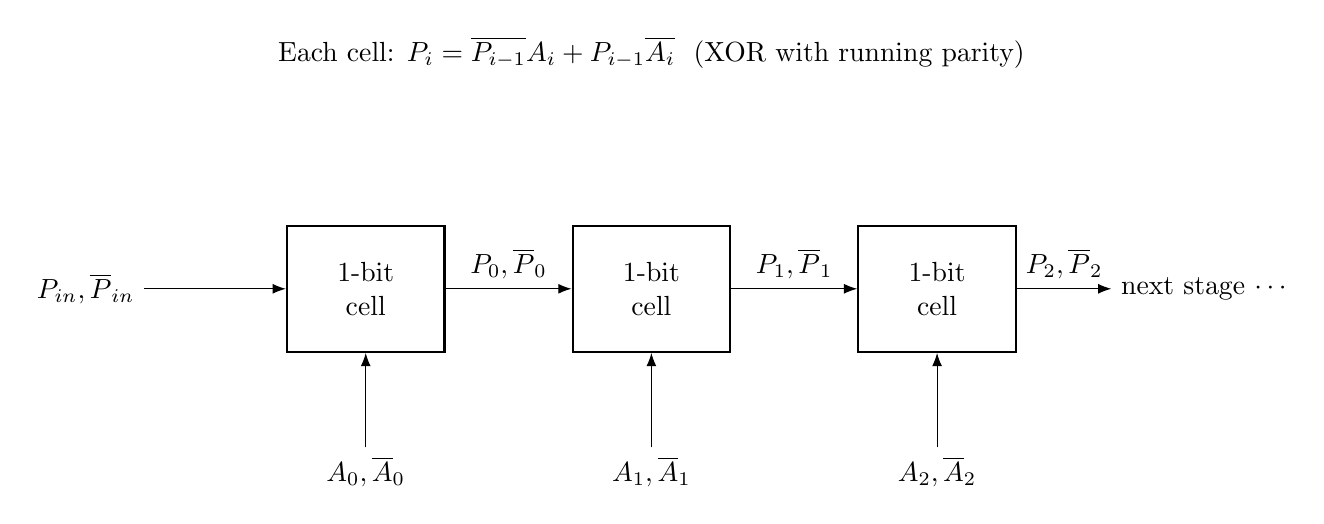
\begin{tikzpicture}[>=Latex, c/.style={draw, thick, minimum width=2cm, minimum height=1.6cm, align=center}]
\node[c] (c0) {1-bit\\ cell};
\node[c, right=1.6cm of c0] (c1) {1-bit\\ cell};
\node[c, right=1.6cm of c1] (c2) {1-bit\\ cell};
\node[right=1.2cm of c2] (next) {next stage $\cdots$};
\draw[->] ($(c0.west)+(-1.8,0)$) node[left]{$P_{in},\overline{P}_{in}$} -- (c0.west);
\draw[->] (c0) -- (c1) node[midway,above]{$P_0,\overline{P}_0$};
\draw[->] (c1) -- (c2) node[midway,above]{$P_1,\overline{P}_1$};
\draw[->] (c2) -- (next) node[midway,above]{$P_2,\overline{P}_2$};
\draw[->] ($(c0.south)+(0,-1.2)$) node[below]{$A_0,\overline{A}_0$} -- (c0.south);
\draw[->] ($(c1.south)+(0,-1.2)$) node[below]{$A_1,\overline{A}_1$} -- (c1.south);
\draw[->] ($(c2.south)+(0,-1.2)$) node[below]{$A_2,\overline{A}_2$} -- (c2.south);
\node[align=center] at (c1 |- 0,3.0)
 {Each cell: $P_i=\overline{P_{i-1}}A_i+P_{i-1}\overline{A_i}$ \ (XOR with running parity)};
\end{tikzpicture}
\end{document}
